\subsection{Tables}

A table answer depends on relations: which header governs a cell, which unit applies, and which rows satisfy the question. Table QA methods differ in where they represent and transform these relations. Figure~\ref{fig:table_stages} follows the evidence from a source table to an answer; Table~\ref{tab:table_evidence_routes} locates representative methods along that workflow.

\begin{figure*}[tp]
\centering
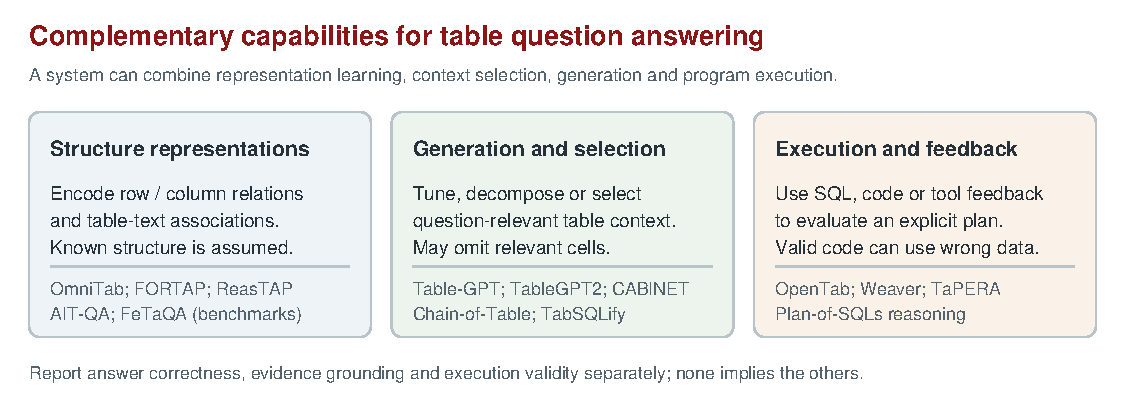
\includegraphics[width=\textwidth]{figs_by_qixingyu/fig05.pdf}
\caption{From a source table to a computed answer. Selection, table transformations and executable programs expose different intermediate objects for inspection.}
\label{fig:table_stages}
\end{figure*}

\subsubsection{Preserving Rows, Columns and Units}

Flattening a table into prose can separate a value from its header or merge unrelated columns. Structure-aware pre-training instead teaches models to associate cell content with row, column and contextual information. TAPAS-style intermediate pre-training~\cite{eisenschlos2020understanding} and OmniTab~\cite{jiang2022omnitab} develop table--question alignment through tabular learning objectives. FORTAP~\cite{cheng2022fortap} uses spreadsheet formulas to connect cell relations with numerical operations. These approaches improve the representation supplied to a reasoning model; they do not replace the initial recovery of structure from a document image.

Representation remains important after pre-training. Structural-noise analysis~\cite{singha2023tabular} shows why changing serialization or disrupting headers can alter an LLM's interpretation of the same cells. A useful input therefore retains header scope, units, missing-value conventions and source coordinates. A clean CSV already supplies much of this information; a scanned financial table requires a separate extraction step. Evaluating the two settings as the same task conceals an important source of error.

\subsubsection{Selecting and Transforming Evidence}

Large tables create a second problem: the relevant evidence may occupy only a few rows. CABINET~\cite{patnaik2024cabinet} uses question-conditioned relevance weighting to suppress distracting content. Selection reduces context, but it must retain the headers and comparison values needed to interpret the remaining cells. Removing an apparently irrelevant unit or denominator can make a compact sub-table unusable.

Other methods transform the evidence rather than only selecting it. Chain-of-Table~\cite{zhang2023chainoftable} maintains a table as intermediate state and updates it through operations such as filtering and aggregation. DePlot~\cite{liu2023deplot} first translates a chart into a table, allowing a language model to reason over extracted values. Their intermediate objects make different errors visible: an incorrect operation in the former, an incorrect visual-to-tabular conversion in the latter.

Instruction tuning changes how a model responds to tabular tasks. Table-GPT~\cite{peng2023table} uses synthetic table-task data, while TableGPT2~\cite{su2024tablegpt2} combines a specialized table encoder with a language decoder. TableGPT2's additional modality is schema- and cell-level tabular information; it should not be confused with directly reading a table image. Such models can also be combined with selection, retrieval or execution rather than treated as alternatives to those mechanisms.

\subsubsection{Computing and Checking the Answer}

Numerical questions benefit from explicit computation. OpenTab~\cite{kong2024opentab} combines table retrieval with generated SQL. TaPERA~\cite{zhao2024tapera} uses content planning and Python execution for long-form table answers; TAT-LLM~\cite{zhu2024tat} addresses discrete reasoning over tables and text. These designs expose operands and intermediate results, making arithmetic easier to inspect than a verbal explanation alone.

Execution nevertheless checks a narrower property than answering the question. A valid SQL query can select the wrong accounting period, and correct subtraction can use an unadjusted value. For a year-on-year margin question, the workflow must connect each value to its year, preserve the percentage unit, apply any restatement and then compute the change. The source table, selected cells, executed operation and final unit should remain linked. The cross-page example in Figure~\ref{fig:cross_page_case} illustrates this dependency.

\begin{table*}[tp]
\centering
\small
\setlength{\tabcolsep}{3pt}
\renewcommand{\arraystretch}{1.18}
\begin{tabular}{@{}p{0.17\textwidth}p{0.25\textwidth}p{0.24\textwidth}p{0.28\textwidth}@{}}
\toprule
Method & Main mechanism & Inspectable object & Essential source check \\
\midrule
TableGPT2~\cite{su2024tablegpt2} & Schema/cell encoding & Table and response & Relevant cells support answer \\
CABINET~\cite{patnaik2024cabinet} & Relevance weighting & Selected content & Required headers survive \\
Chain-of-Table~\cite{zhang2023chainoftable} & Iterative table operations & Intermediate tables & Operations match question \\
DePlot~\cite{liu2023deplot} & Chart-to-table conversion & Extracted values & Values match chart \\
OpenTab~\cite{kong2024opentab} & Retrieval and SQL & Table, SQL, result & Correct table and columns \\
TaPERA~\cite{zhao2024tapera} & Planning and Python & Plan, program, output & Inputs and plan match source \\
\bottomrule
\end{tabular}
\caption{Table QA methods compared by the evidence object they expose. The final column identifies checks that remain beyond successful generation or execution.}
\label{tab:table_evidence_routes}
\end{table*}

\subsubsection{Choosing a Table QA Workflow}

The input and question should determine the workflow. For a small, clean table, a direct reader with arithmetic execution may suffice. For a wide table, select a compact sub-table while retaining its schema. For an open collection, retrieve the table before reasoning over its cells. For image-based evidence, inspect extraction quality before attributing an error to downstream reasoning. Table~\ref{tab:table_evidence_routes} supports this choice without collapsing representation, selection and execution into a single model ranking.
